% ==============
% PARAMETRAGES
% à compiler en pdfLaTeX
% ==============

% GENERAL
%  type de document rapport, chapitre commence en page impaire ou paire indifféremment
\documentclass[twoside,a4paper,11pt,frenchb,openany]{report}  
%  type de document, chapitre commence en page impaire
%\documentclass[twoside,a4paper,12pt,frenchb,openright]{report} 
\title{Etat de l'art du projet de recherche}
\author{Stephane Robin}
\date{\today}

% IMPORTATION DE LIBRAIRIES
\usepackage{amssymb}  % symboles
\usepackage{amsmath}  % symboles mathématiques
\usepackage{amsfonts}  % polices de caractères
\usepackage{amscd}
\usepackage{amsthm}  % symboles mathématiques pour redéfinir les théorèmes
\usepackage[all,cmtip]{xy}
\usepackage{array}  % tableaux
\usepackage[frenchb]{babel}  % langue française
\usepackage{bm}  % caractères grecs
\usepackage{calc}
\usepackage{enumitem} % listes
\usepackage{eurosym}  % symbole euro
\usepackage{euscript}
\usepackage{fancybox}  % boîtes
\usepackage{float}  % images flottantes
\usepackage[T1]{fontenc}  % LaTeX modele
\usepackage[top=3.1cm,bottom=2.7cm,left=2.2cm,right=2.2cm,dvips]{geometry}  % marges
\usepackage{graphicx}  % insertion images
\usepackage[utf8]{inputenc}  % accents
\usepackage{mathrsfs}  % symboles mathématiques
\usepackage{mathtools}  % outils mathématiques
\usepackage{mdframed} % box autour des theoremes
\usepackage{pst-plot, pstricks}
\usepackage{pstricks-add}
\usepackage{rotating}
\usepackage{srcltx}
\usepackage{textcomp}   % caracteres complementaires
\usepackage{titlesec}  % sections
\usepackage{titletoc}  % table de contents
%\usepackage[nottoc,notlof,notlot]{tocbibind}  % bibliothèque
\usepackage{verbatim}  % caracteres non interpretes
\usepackage{wrapfig}  % pour inserer les figures dans du texte

% COULEURS
\definecolor{couleurTitre}{RGB}{64,128,128}  % doit être défini avant xcolor
\definecolor{couleurUrl}{RGB}{127,62,0}
\usepackage{xcolor}  % couleurs
%\definecolor{amber}{rgb}{1.0,0.49,0.0} % couleur non utilisee
%\definecolor{greyish}{rgb}{52.0,160.0,157.0} % couleur non utilisee
%\definecolor{theoremeCouleur}{rgb}{224.0,90.0,67.0} % couleur non utilisee
	
% LISTES
\renewcommand{\labelitemi}{$\bullet$}  % symboles de listes
\frenchbsetup{StandardLists=true}  % style de bullets

% IMAGES
\usepackage{caption}  % insertion d'images
\usepackage[font=footnotesize,labelfont=bf]{caption}  % légendes des images
\renewcommand{\thefigure}{\arabic{section}.\arabic{figure}}  % numérotation des images
\usepackage{subcaption}

% HYPERLINKS
\usepackage{hyperref}
\hypersetup{
colorlinks=true,
linkcolor=couleurUrl,
citecolor=couleurUrl,
urlcolor=couleurUrl
}

% LIGNES
\usepackage{parskip}
%\setlength\parskip{\baselineskip} % joint a la suppression de l'espace horizontal
%\setlength{\parindent}{0cm} % supprime l'espace horizontal en debut de ligne

% HEADINGS AND FOOTERS
\usepackage{fancyhdr}  % entete
\pagestyle{fancy}  % la page accepte les entetes et pieds de page
\renewcommand{\headrulewidth}{0pt}
\fancyhead[L,R,C]{}
%\fancyhead[LE]{} % pages paires header gauche
%\fancyhead[CE]{} % pages paires header centre
%\fancyhead[RE]{Le théorème de Pythagore} % pages paires header droit
%\fancyhead[LO]{Le théorème de Pythagore} % pages impaires header gauche
%\fancyhead[CO]{} % pages impaires header centre
%\fancyhead[RO]{} % pages impaires header droit
%\fancyfoot[c]{\textcolor{gray}{\thepage}}  % pied de page
%\fancyfoot[L,R,C]{} % forcing footer empty

% REDEFINITION DU STYLE DE THEOREM
\newmdtheoremenv[  % definitions
linewidth=5,
leftline=true,
rightline=false,
bottomline=false,
topline=false,
leftmargin=0,
rightmargin=0,
backgroundcolor=couleurTitre!20,
linecolor=orange!70,
innertopmargin=21pt,
skipabove=\topskip,
ntheorem=true]{definition}{Définition}

\newmdtheoremenv[  % theoremes
linewidth=5,
leftline=true,
rightline=false,
bottomline=false,
topline=false,
leftmargin=0,
rightmargin=0,
backgroundcolor=couleurTitre!20,
linecolor=orange!70,
innertopmargin=10pt,
skipabove=\topskip,
ntheorem=true]{theorem}{}

\newmdtheoremenv[  % proprietes
linewidth=5,
leftline=true,
rightline=false,
bottomline=false,
topline=false,
leftmargin=0,
rightmargin=0,
backgroundcolor=couleurTitre!20,
linecolor=orange!70,
innertopmargin=21pt,
skipabove=\topskip,
ntheorem=true]{property}{Propriété}

\newmdtheoremenv[  % propositions
linewidth=5,
leftline=true,
rightline=false,
bottomline=false,
topline=false,
leftmargin=0,
rightmargin=0,
backgroundcolor=couleurTitre!20,
linecolor=couleurTitre!70,
innertopmargin=21pt,
skipabove=\topskip,
ntheorem=true]{proposition}{Proposition}

\newmdtheoremenv[  % corollaires
linewidth=5,
leftline=true,
rightline=false,
bottomline=false,
topline=false,
leftmargin=0,
rightmargin=0,
backgroundcolor=couleurTitre!20,
linecolor=couleurTitre!70,
innertopmargin=21pt,
skipabove=\topskip,
ntheorem=true]{corollary}{Corollaire}

\newmdtheoremenv[  % lemmes
linewidth=5,
leftline=true,
rightline=false,
bottomline=false,
topline=false,
leftmargin=0,
rightmargin=0,
backgroundcolor=couleurTitre!20,
linecolor=couleurTitre!70,
innertopmargin=21pt,
skipabove=\topskip,
ntheorem=true]{lemma}{Lemme}

% NUMEROTATION DES CHAPITRES-SECTIONS
\renewcommand{\theequation}{\arabic{chapter}.\arabic{equation}}  % equations
%\renewcommand{\theequation}{\thesection\arabic{equation}}  % equations
%\numberwithin{equation}{section}  % equations

%\renewcommand{\thepart}{\Alph{part}}  % parties
\renewcommand{\thechapter}{\arabic{chapter}.}  % chapitres
\renewcommand{\thesection}{\arabic{section}.}  % sections
\renewcommand{\thesubsection}{\arabic{section}.\arabic{subsection}.}  %  sous-sections
\renewcommand{\thesubsubsection}{\arabic{section}.\arabic{subsection}.\arabic{subsubsection}.}  % sous-sous-sections

\renewcommand{\thedefinition}{\arabic{chapter}.\arabic{definition}}  % definitions
\renewcommand{\theorem}{}  % theoremes
\renewcommand{\theproperty}{\arabic{chapter}.\arabic{property}}  % property
\renewcommand{\theproposition}{\arabic{chapter}.\arabic{proposition}}  % propositions
\renewcommand{\thecorollary}{\arabic{chapter}.\arabic{corollary}}  % corollaires
\renewcommand{\thelemma}{\arabic{chapter}.\arabic{lemma}}  % lemmes
\setcounter{secnumdepth}{4}  % profondeur de numérotation

% FORMAT DES SECTIONS-TITRES
\titleformat{\section}{\normalfont\normalsize\bfseries}{\textcolor{couleurTitre}{\thesection}}{1em}
{\normalfont\large\bfseries\scshape\textcolor{couleurTitre}} % format de titre de section
\titleformat{\subsection}{\normalfont\normalsize\bfseries}{\textcolor{couleurTitre}{\thesubsection}}{1em}
{\normalfont\normalsize\bfseries\textcolor{couleurTitre}}  % format de titre de sous-section
\titleformat{\subsubsection}{\normalfont\normalsize\bfseries\itshape}{\textcolor{couleurTitre}{\thesubsubsection}}{1em}
{\normalfont\normalsize\bfseries\itshape\textcolor{couleurTitre}}  % format de titre de sous-sous-section

\makeatletter

%\renewcommand{\@chapapp}{}  % le mot `chapitre'' n'apparait plus en titre de chapitre
\renewcommand\l@section{\@dottedtocline{1}{0em}{5.0em}}  % espacement dans le titre d'une section
\renewcommand\l@subsection{\@dottedtocline{1}{2.5em}{1.5em}}  % espacement dans le titre d'une sous-section
\renewcommand\l@subsubsection{\@dottedtocline{1}{5em}{2.5em}}  % espacement dans le titre d'une sous-sous-section

\makeatother

% ==============
% DEBUT DU DOCUMENT
% ==============

\begin{document}

\maketitle

\section{Introduction}

Le présent document cherche à définir les fondements sur lesquels va reposer le stage et en particulier de connaître l'état actuel des connaissances concernant l'analyse bioinformatique du locus CRISPR-Cas chez \textit{Mycobacterium tuberculosis}.

L'objectif du stage est de comprendre les liens entre les sept lignées de \textit{tuberculosis} et les alternances de gènes et espaceurs du locus CRISPR-Cas, au moyen d'outils développés au sein de l'équipe AND de l'Université de Franche Comté.


% OUT OF AFRICA MIGRATION ========================================================
\section{Evolution de la branche humaine de la tuberculose}

Le développement des maladies s'adapte à la densité de population concernée. En effet, auprès d'une foule dense, les infections se répandent plus largement et deviennent plus virulentes, alors qu'auprès d'une population moins importante, elles ont une croissance plus faible, laissant place parfois à des périodes où les infections restent latentes.

Une période charnière dans l'histoire de l'humanité est la transition démographique du Néolithique, qui a vu il y a 10 000 ans, suite à l'apparition de l'agriculture et de l'élevage, un accroissement de la population, favorisant la naissance de nombreuses maladies. Les maladies humaines plus anciennes se développaient auprès de populations moins denses et produisaient des phases chroniques de latence et de réactivation permettant aux populations infectées de survivre.

La tuberculose conjugue ces deux modèles de maladie. En effet, elle a montré à travers les âges des périodes de réactivation, elle dépend fortement de la densité de population et son mode de transmission aérosol s'est parfaitement adapté aux foules.

% The global diversity of human-adapted MTBC

L'analyse phylogénique\footnote{\textbf{Phylogénie} : étude des liens entre espèces apparentées, permettant de retracer les principales étapes de l'évolution des organismes depuis un ancêtre commun.} de Comas et al.\cite{comas} se base exclusivement sur l'étude du génome complet de toutes les lignées connues de tuberculose en utilisant les SNPs pour construire les relations entre les différentes branches. Les résultats obtenus rejoignent de précédentes études effectuées à partir d'autres marqueurs, et confirment l'existence de sept principales lignées de tuberculose. On remarque en particulier que plusieurs branches d'origine animale se sont regroupées avec la lignée 6 d'Afrique de L'Ouest 2, et que les lignées modernes 2, 3 et 4 d'Europe ont des origines proches. Par ailleurs, seuls 1,1 \% des SNPs sont homoplastiques, ce qui suggère que la structure de la tuberculose favorise les clonages plutôt que les recombinaisons entre branches.  

% African origin and co-divergence of MTBC with modern humans

L'étude phylogénique de Comas et al.\cite{comas} corrobore les connaissances actuelles selon lesquelles la tuberculose est originaire d'Afrique. Par ailleurs, s'appuyant sur les origines africaines de l'espèce humaine, elle cherche également à déterminer l'ancienneté de l'association entre la tuberculose et son hôte humain. L'analyse des divergences des génomes de la tuberculose est comparée à celle d'une arborescence génétique déjà établie à partir de mitochondries de l'être humain. 

% Age of the association of MTBC and humans

Les similitude relevées montrent que la tuberculose a infecté les premiers hommes d'Afrique. Pour aller plus loin, l'étude de Comas et al. a tenu compte de 3 dates importantes dans l'évolution de l'être humain qui ont été reportées sur l'analyse phylogénique de la tuberculose des lignées 5 et 6 d'Afrique de l'Ouest :

- l'émergence de l'homo sapiens correspondant au MTBC-185\footnote{\textbf{MTBC} : Mycobacterium Tuberculosis Complex.},\\
- l'émergence du halogroupe mitochondriaque de la lignée 3 chez l'homme correspondant au MTBC-70,\\
- le début de la transition démographique du Néolithique correspondant au MTBC-10.

La branche MTBC-70 a révélé des corrélations avec l'histoire de l'humanité, telle qu'elle a été décrite par l'archéologie, en montrant l'apparition des sept différentes lignées de tuberculose :

- il y a 73 000 ans, apparition des lignées 5 et 6 correspondant à une 1ère migration humaine importante vers l'Afrique de l'Ouest,\\
- il y a 67 000 ans, apparition de la lignée 1 correspondant à une migration humaine importante autour de l'Océan Indient,\\
- il y a 64 000 ans, apparition de la lignée 7 concernant une population qui est restée en Afrique ou est revenue en Afrique après une 1ère migration,\\
- il y a 46 000 ans, apparition de la lignée 4 correspondant à une migration humaine importante vers l'Europe,\\
- il y a 42 000 ans, apparition des lignées 2 et 3 correspondant à une migration humaine importante vers l'Asie de l'Est et l'Asie Centrale. 

En revanche, la branche MTBC-185 suggère l'apparition de mutations à partir de lignées africaines il y a 174 000 ans, c'est à dire que la dispersion de la tuberculose précèderait celle de l'homo sapiens.

% Neolithic co-expansion of MTBC and humans

Dans tous les cas, la tuberculose aurait infecté l'espèce humaine et évolué conjointement avec elle depuis 70 000 ans, mais son apparition serait antérieure à la transition démographique du Néolithique.

La base de données de tuberculose étudiée de façon probabiliste par Comas et al. montre que le Néolithique a fortement contribué à l'expansion de la maladie il y a 10 000 ans grâce à l'augmentation de la densité de population, à la probabilité de co-infection avec d'autres maladies dépendantes de la densité de population, et non pas grâce à la possibilité pour la tuberculose de muter d'une variété animale vers une variété humaine. En effet, l'analyse phylogénique de la tuberculose montre que les branches humaines ont divergé des branches animales avant le Néolithique.

Le Néolithique n'était pas la seule période où l'augmentation de la population fut importante, toutefois la concentration de population qui s'en est suivie a permis l'apparition auprès de la tuberculose de caractères fortement dépendants de la densité de population qu'elle affecte. Le Néolithique a donc marqué un tournant dans l'histoire de la tuberculose qui a alors commencé à conjuguer les deux modèles de maladie, dépendant de la densité de population et chronique par périodes de réactivation.

% The evolutionary history of MTBC at a regional scale

 % Conclusion

Il faut donc considérer que la co-existence de la tuberculose avec l'espèce humaine depuis des milliers d'années a conduit la maladie à s'adapter aux changements du génome humain et inversement. Les prochaines études sur la tuberculose devraient donc se concentrer sur des génomes complets de la tuberculose et de l'être humain choisis en rapport à leurs associations.

Par ailleurs, une étude récente de Perry S. et al.\cite{perry1, perry2} suggère que l'infection d'une organisme par l'Helicobacter Pylori pourrait protéger de la tuberculose sous sa forme active. A contrario, nous ne savons pas si la tuberculose latente pourrait protéger contre les ulcers et les cancer de l'estomac causés par l'Helicobacter Pylori.



%  GLOBAL EXPANSION OF MTBC LINEAGE 4 =============================================

\section{L'expansion de la lignée 4 de tuberculosis}





% SPOLPRED ==========================================================

\section{Le locus CRISPR-Cas}

% Le locus CRISPR Cas

\subsection{Description}

Le locus CRISPR \textit{Clusterd Regularly Interspaced Short Palindromic Repeats} est une famille de séquences répétées dans l'ADN formant un palindrome. Chaque série de répétition contient entre 21 et 37 bp, régulièrement espacées par des \textit{spacers} de 20 à 40 bp. Cette structure répétée se trouve à l'état naturel chez 40\% des bactéries (dont le MTBC) et la plupart des archées. Elle est héritable par transmission aux cellules filles et se conserve donc pour une même espèce. Les locus CRISPR sont généralement adjacents aux gènes Cas, dont ils sont séparés par une séquence de 300 à 500 bp, appelée leader qui contrôle à la fois la l'acquisition de l'ADN viral par les spacers et la fabrication de protéines. Les gènes Cas produisent des protéines aux fonctionnalités différentes et notamment les enzymes capable de couper l'ADN en vue de leur réparation.

Ces séquences incorporent dans les spacers des fragments d'ADN de bactériophages qui ont déjà infecté la bactérie qui sont stockés en vue de détecter et de détruire l'ADN de bactériophages similaires en cas d'infection ultérieure. Par conséquent, CRISPR-Cas est un système immunitaire naturel utilisé par les bactéries pour se protéger des infections virales. 

\begin{figure}
\centering
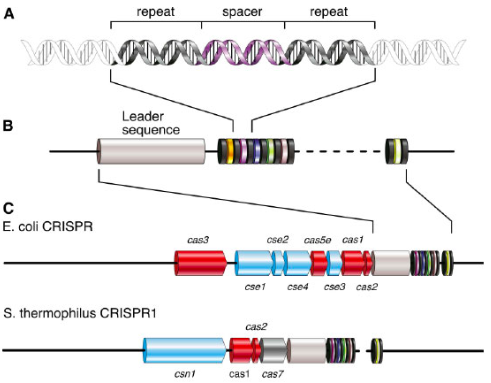
\includegraphics[scale=0.6]{crispr.png}
\caption{Structure du locus CRISPR-Cas, d'après\\ \url{https://www.sinobiological.com/crispr-locus.html}}
\end{figure}


\subsection{Fonctionnement du système CRISPR-Cas}

Le système CRISPR-Cas fonctionne de la façon suivante : lorsque la bactérie détecte la présence d'ADN ou d'ARN d'un virus, elle produit une protéine appelée Cas9 capable de couper l'ADN, une séquence d'ARN CRISPR notée crARN correspondant à celle de l'ADN du virus et une séquence d'ARN traceur notée trARN qui joue le rôle d'un guide ARN. Lorsque trARN trouve sa cible parmi le genome du virus, Cas9 sectionne son ADN, désactive le virus, puis insère un fragment de l'ADN du virus dans un \textit{spacer} du génome de la bactérie afin de conserver en mémoire une trace de ce virus afin de le reconnaître lors d'une éventuelle nouvelle infection. Les espaceurs servent donc de banque de mémoire en conservant l'ADN des virus qui ont attaqué la bactérie.

Les différentes étapes du système CRISPR-Cas sont donc les suivantes :

1. adaptation de l'ADN de la bactérie à l'ADN ou ARN du bactériophage, en incorporant des portions d'ADN du virus dans les spacers de la bactérie,\\
2. création de crRNA et trRNA à partir de la nouvelle séquence d'ADN légèrement modifiée suite à l'infection virale. Avec l'aide de Cas9, trRNA et crRNA coupent l'ADN cible à un emplacement spécifique.\\
3. création d'enzymes permettant de lutter contre le bactériophage.

Mécanisme moléculaire :

Les systèmes CRISPR utilisent les gènes cas1 et cas2 qui sont impliqués dans l'intégration, en tant que spacer de fragments de gènes étrangers dans le CRISPR.

Trois types de systèmes CRISPR-Cas sont connus :

les systèmes de types I, utilisent un complexe Cascade pour cliver les transcrits de CRISPR au niveau des épingles. Lorsqu'un complexe Cascade/spacer s'associe à un ADN cible (reconnaissance par hybridations) il recrute la protéine Cas3 qui clive un brin de l'ADN cible ;
les systèmes de types II, utilisent la RNAse III pour séparer les répétitions des transcrits. La protéine Cas9 s'associent avec un fragment de transcrit et, lors de la reconnaissance d'un ADN cible, Cas9 clive les 2 brins de cet ADN ;
les systèmes de type III, utilisent la protéine Cas6 pour cliver les transcrits de CRISPR au niveau des épingles, les segments de transcrits obtenus s'associent avec un complexe Cas10. Ce système requiert qu'il y ait transcription de l'ADN cible, le complexe Cas10/spacer clive alors un brin de l'ADN cible (brin non transcrit), ainsi que l'ARN en cours de transcription.

% REVOIR VIDEO POUR COMPARER

La technologie CRISPR-Cas9 s'inspire du système du même nom a d'abord été utilisée pour typer les souches bactériennes, suivant une technique appelée \textit{spoligotyping}. CRISPR-Cas9 est actuellement principalement employé comme ciseau moléculaire afin d'éditer le génome et d'introduire localement des modifications génétiques.

% Spoligotyping

\subsection{Le spoligotyping}

Le spoligotyping, \textit{Spacer Oligonucleotide Typing}, repose sur la détection de séquences répétitives, ou \textit{Direct Repeat} DR, trouvées entre les gènes d'un agent infectieux au sein d'un locus CRISPR-Cas. Pour ce faire, la région DR d'un isolat à tester subit un traitement PCR ou celui d'une puce à ADN pour dévoiler un motif de taches correspondant aux spacers. La comparaison de ces motifs permet la différentiation des souches. Ainsi, le locus CRISPR-Cas permet le génotypage des souches de tuberculosis.

Xia E. et al. et Coll F. et al. expliquent dans leurs articles \cite{xia, coll} que la séquence répétée DR au sein du locus CRISPR de tuberculosis mesure 36 bp. Les spacers, quant à eux mesurent de 34 à 41 bp. Le polymorphisme entre les différentes souches résulte des variations et de l'identité des spacers. La classification de MTBC utilise un groupe de 43 bit représentant la présence ou l'absence d'espaceurs dans le locus CRISPR, qu'on appelle spoligotype.

Les spoligotypes ainsi obtenus peuvent être partagées entre laboratoires et corroborent les résultats obtenus à partir d'autres marqueurs génétiques. Ces données numériques permettent de bien différencier les souches de tuberculosis et sont de moindre coût comparativement à d'autres méthodes. Cependant, le spoligotyping éprouve des difficultés à bien différencier les souches au sein de grandes familles de souches telles que la branche Beijing.

Le spoligotyping a permis de fournir une image globale de la diversité des souches de tuberculosis.

% Normalisation

\subsection{Vers une normalisation des spoligotypes}

Au début du spoligotyping, il n'existait pas de norme pour décrire les motifs formés par les spacers ou simplement les numéroter. Chaque laboratoire utilisait son propre système de numérotation accompagné d'un schéma descriptif du motif. Ce manque de normalisation entravait les possibilités de comparaison des résultats obtenus et le développement d'une vision mondiale de l'évolution de MTBC. Une méthode standardisée de description des spoligotypes a été proposée en 2001 par Dale JW dans son article \cite{dale}. 

Tout d'abord, une base de données centralisée regroupant tous les motifs connus et de leurs numérotations jusqu'à présent associées existe au RIVM Rijksinstituut voor Volksgezondheid en Milieuhygiene, Bilthoven, Netherlands. Elle peut être consultée au \url{http://www.caontb.rivm.nl}. A partir de 2001, les nouveaux motifs devraient prendre un unique format de numérotation pour être répertoriés dans cette base de données. Toutefois, cela nécessite l'interrogation systématique de la base de données et la comparaison avec les éléments déjà existants pour chaque nouveau spoligotype. Pour éviter cette perte de temps, de nombreux laboratoires utilisent des systèmes rationnels avec des codes descriptifs assignés à chaque isolat. 

Dale JW et al. dans leur article \cite{dale} proposent d'utiliser exclusivement un système rationnel octal ou hexadécimal, sachant qu'il est aisé de passer de l'un à l'autre et qu'il est également facile de retrouver l'état initial binaire. Ainsi, les motifs de spoligotype comprenant 43 bits seraient réduits dans le système octal en 14 groupes de 3 bits auquel s'ajouterait un unique bit, ce qui donnerait finalement un ensemble de 15 chiffres en écriture octale. En ce qui concerne le système hexadécimal, les motifs de 43 bits seraient réduits en 6 groupes de 8 bits avec un dernier groupe ne comprenant que 3 bits, soit 6 groupes de 2 chiffres hexadécimaux. Notons que un bit symbolise dans ce cas la présence ou l'absence d'une espaceur dans le locus étudié. Un exemple est donné ci-dessous dans le document \cite{dale} publié par Dale et al.

\begin{figure}

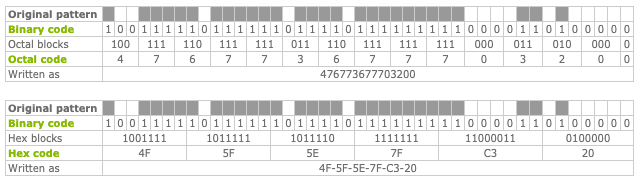
\includegraphics[scale=0.6]{hexa.png}
\caption{Exemple de système rationnel octal et hexadécimal, d'après \textit{SpoTyping:\\ fast and accurate in silico Mycobacterium spoligotyping from sequence reads}}
\end{figure}

% Spolpred et SpoTyping

\subsection{Quel outil informatique choisir pour le spoligotyping ?}

Les technologies PCR de génotypage utilisent toujours différents marqueurs tels que les SNPs pour obtenir en laboratoire des résultats fiables. Des logiciels informatique de prédiction du génotype ont également fait leur apparition pour optimiser les coûts et le gain de temps. Ils offrent un outil de comparaison des résultats obtenus expérimentalement et in silico.

SpolPred est un logiciel de prédiction rapide et précis des spoligotypes de tuberculosis à partir de séquences génomiques courtes appelées reads. Cet outil développé par Preston M. fonctionne efficacement avec des reads provenant de plateformes telles que Illumina GAII ou HiSeq. SpolPred utilise des fichiers de séquences de reads simples ou par paires au format FASTQ, pour produire une prédiction de spoligotype au format octal qui est comparée au spoligotype correspondant dans la base SITVITWEB\footnote{L'application en ligne SITVIT2 \url{http://www.pasteur-guadeloupe.fr:8081/SITVIT2/index.jsp} est une mise à jours de SITVIT WEB, présenté dans l'article\cite{demay}, qui permet d'analyser des data au regard des markers Spoligotypes, ETR et MIRU-VNTR afin d'en trouver notamment l'origine.}.

Dans leur étude, Coll F. et al.\cite{coll} montrent en 2012 l'utilité de SpolPred en comparant les spoligotypes obtenus par le logiciel avec les résultats de laboratoire. Ils dévoilent également les limites de la méthode expérimentale qui a répertorié cinq faux spoligotypes, alors que SpolPred YYYYY. Par ailleurs, il apparaît que SpolPred offre plus de précision, plus de rapidité et des résultats pratiquement identiques à ceux obtenus avec la méthode bioinformatique par assemblage, consistant à fusionner des fragments d'ADN issus d'une plus longue séquence afin de reconstruire la séquence originale, à l'aide du logiciel Velvet développé en 2008.

Toutefois, d'après l'étude de Xia et al.\cite{xia}, la précision de SpolPred est fortement réduite lorsque les reads n'ont pas une taille uniforme, comme par exemple lorsqu'ils proviennent de séquençages Ion Torrent ou de la plateforme de diagnostique clinique Illumina MiSeq. Ainsi, lorsque les reads ne sont pas uniformes, la précision des résultats dépend fortement de leurs tailles et donc du choix initial fait par l'opérateur. Par ailleurs, SpolPred demande à l'utilisateur de spécifier la direction de lecture des reads, et le logiciel n'utilise donc qu'une partie des informations fournies par les reads.

Une problématique de SpolPred en 2020 est que le logiciel n'est plus disponible au public. En effet, une visite sur le site officiel \url{http://www.pathogenseq.org/spolpred} fourni comme référence dans le document \cite{coll} de Coll F. et al. montre que le nom de domaine est à vendre. Preston M., qui a fait partie de l'équipe de rechercher de Coll F. pour le développement de SpolPred, a bien créé un site \url{https://www.mybiosoftware.com/spolpred-predict-the-spoligotype-from-raw-sequence-reads.html} proposant le téléchargement du logiciel, mais le lien est actuellement inactif.

Une alternative à SpolPred est SpoTyping présenté en 2016 dans l'article \cite{xia} de Xia et al. comme étant 20 à 40 fois plus rapide que SpolPred pour prédire avec précision des spoligotypes de tuberculosis à partir de reads de taille uniforme ou variable. Par ailleurs, SpoTyping lit chaque read dans les deux directions en exploitant complètement les informations fournies. SpoTyping réduit la durée des recherches en intégrant l'algorithme BLAST\footnote{\textit{BLAST Basic Local Alignment Search Tool} : logiciel basé sur l'algorithme du même nom qui détecte des régions similaires entre plusieurs séquences biologiques. Le programme compare les séquences de nucléotides aux séquences contenues dans la base de données BLAST pour fournir des résultats statistiquement significatifs.} dans ses calculs. Il compare les isolats testés avec ceux ayant le même spoligotype dans la base de données mondiale de marqueurs moléculaires de la tuberculose SITVIT\footnote{La base de données SITVIT comprend les spoligotypes de tuberculosis, ainsi que les marqueurs utilisés pour les détecter MIRU12, VNTR, SIT, MIT, VIT, les différentes branches de MTBC, les pays d'origine et l'année de découverte.}, qui regroupe les données épidémiologiques associées à des isolats de même spoligotype.

SpoTyping utilise des fichiers de séquences de reads simples ou par paires au format FASTQ et des fichiers de séquences complètes de génomes ou de contigs assemblés au format FASTA. Le séquences de reads sont regroupés en une unique séquence continue au format FASTA pour être ensuite soumis à l'algorithme BLAST qui détecte les régions similaires. Finalement la base de données SITVIT permet d'identifier les isolats ayant le même spoligotype. SpoTyping est limité à une lecture de 250 Mbp au sein des séquences de reads testées, lors de l'utilisation du swift mode qui accélère le temps de traitement.

SpoTyping propose un rapport statistique permettant de résumer le rapprochement avec les spoligotypes trouvés dans la base de données SITVIT, ainsi qu'une estimation du nombre de correspondances positives pour chaque spacer.

L'étude de Iwai H: et al. \cite{iwai} montre l'intérêt d'une analyse de MTBC à l'aide de serveurs, appelée CASTB, et notamment le spoligotyping. Le Webserver fournit une vue complète des données, mais les performances de chaque outil utilisé ne sont pas décrites dans l'article. Il est probable que le spoligotyping prenne plus de temps en passant par un serveur suite au problème de disponibilité des données et aux lenteurs de téléchargement de ces données. Il semblerait que SpoTyping, de par sa configuration locale, puisse fournir un résultat en une minute.

\begin{figure}
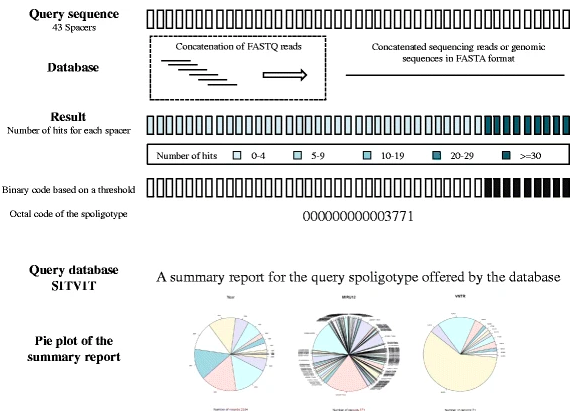
\includegraphics[scale=0.6]{spotyping.png}
\caption{Exemple de fonctionnement de SpoTyping, d'après \textit{SpoTyping:\\ fast and accurate in silico Mycobacterium spoligotyping from sequence reads}}
\end{figure}

\textit{Spécifications techniques}, d'après \url{https://github.com/xiaeryu/SpoTyping-v2.0/blob/master/SpoTyping-v2.0-commandLine/SpoTyping-README.pdf}

SpoTyping peut s'exécuter sur les principaux systèmes d'exploitation, contrairement à SpolPred qui utilise exclusivement Linux. Il se présente à la fois sous forme de script et sous forme d'application avec une interface graphique.

SpoTyping est un logiciel open-source qui peut se télécharger gratuitement à l'adresse \url{https://github.com/xiaeryu/SpoTyping-v2.0}.

SpoTyping nécessite l'utilisation de Python2.7 et BLAST.\\
Le fichier obtenu propose une prédiction de spoligotype au format de code binaire et octal.\\
Le fichier log obtenu contient de nombre de correspondances positives des résultats de BLAST pour chaque séquence de spacer.\\
Le fichier xls Excel obtenu fournit le resultat de la recherche de spoligotype auprès de la base de données SITVIT WEB. (actuellement SITVIT2)

Il est recommandé d'utiliser le swift mode paramétré par défaut si le débit de séquençage est inférieur à 135 Mbp.\\
Pour les débits de séquençage inférieurs à 135 Mbp ou supérieurs à 1260 Mbp, les seuils doivent être réglés entre 0.018 et 0.1486 fois la profondeur de lecture estimée pour les hits sans erreur, et entre 0.018 et 0.1488 fois la profondeur de lecture estimée pour les hits tolérant une erreur. Notons que la profondeur de lecture est définie par le débit de séquençage divisé par 4 500 0000 qui correspond à l'estimation de la longueur d'un génome de MTBC.

















% problème rencontré par Coll à faire ressortir





% LEXIQUE =============================================

\section{Lexique}



\textbf{Epidémiologie} : discipline scientifique qui étudie les problèmes de santé dans les populations humaines, leur fréquence, leur géographie ainsi que les facteurs influants.

\textbf{Annotation des gènes} : processus permettant d'identifier l'emplacement des gènes dans l'ADN, de déterminer leurs fonctions et leurs possibles interactions.

\textbf{Génome} : ensemble de l'information génétique d'un organisme. Par extension, le génome se réfère aussi au support physique de cette information génétique, la macromolécule d'ADN.

\textbf{Séquençage du génome} : consiste, par des méthodes chimiques ou de biologie moléculaire, à déterminer l'ordre des nucléotides de l'ADN.

\textbf{bp} : une paire de base est l'appariement de 2 bases nucléiques situées sur 2 brins complémentaires d'ADN, reliées par des ponts d'hydrogène.

\textbf{SNP Single Nucleotide Polymorphism} : il s'agit de la variation ou polymorphisme d'une seule paire de bases du génome entre organismes d'une même espèce.

\textbf{Haplogroupe} : groupe possédant les mêmes caractères génétiques et partageant un ancêtre commun suivant une mutation SNP.

\textbf{Homologie} : similitude de caractères observée chez deux espères différentes, provenant de l'héritage d'un ancêtre commun. 

\textbf{Homoplasie} : similitude de caractères chez différentes espèces, qui ne provient pas d'un ancêtre commun, mais peut par exemple provenir d'une adaptation à l'environnement.

\textbf{Mitochondrie} : centrale énergétique des cellules qui contribue à la production d'ATP.

\textbf{Polymère} : macromolécule répétant un même motif structural.

\textbf{PCR Polymerase Chain Reaction} : méthode de réaction en chaîne utilisant un polymère pour dupliquer en grand nombre une séquence d'ADN spécifique. La méthode PCR repose sur le cycle thermique, qui expose les séquences à des cycles répétés de chauffage et de refroidissement pour permettre différentes réactions dépendantes de la température comme la fusion de l'ADN et la réplication de l'ADN par les enzymes. La méthode PCR utilise deux agents principaux : les polymères d'ADN et les \textit{primers}.

\textbf{puce à ADN} : ensemble de molécules d'ADN fixées sur une petite surface solide permettant de mesurer le niveau d'expression d'un grand nombre de gènes simultanément, ou de déterminer le génotype de plusieurs régions d'un génome.

\textbf{Enzyme de restriction} : protéine capable de couper un fragment d'ADN au niveau d'une séquence de nucléotides caractéristique appelée site de restriction. Chaque enzyme de restriction reconnaît ainsi un site spécifique.


% =========
% BIBLIOTHEQUE
% =========
\bibliographystyle{}
\renewcommand{\bibname}{Références}
\begin{thebibliography}{10}
\bibitem{comas}Comas I. et al. \textit{Out-of-Africa migration and Neolithic coexpansion of Mycobacterium tuberculosis with modern humans}\\ \\

\bibitem{coll}Coll F. et al., \textit{SpolPred : rapid and accurate prediction of Mycobacterium tuberculosis spoligotypes from short genomic sequences. Bioinformatics. 2012;28(22):2991–3}\\ \\

\bibitem{brynildsrud}Brynildsrud O.B. et al., \textit{Global expansion of Mycobacterium tuberculosis lineage 4 shaped by colonial migration and local adaptation}\\ \\

\bibitem{driscoll}Driscoll J. R., \textit{Spoligotyping for molecular epidemiology of the Mycobacterium tuberculosis complex}\\ \\

\bibitem{jinek}Jinek M. et al, \textit{A programmable dual-RNA-guided DNA endonuclease in adaptive bacterial immunity}\\ \\

\bibitem{gori}Gori A. et al, \textit{Spoligotyping and Mycobacterium tuberculosis}\\ \\

\bibitem{perry1}Perry S. et al., \textit{Infection with Helicobacter pylori is associated with protection against tuberculosis}\\ \\

\bibitem{perry2}Perry S. et al, \textit{The immune response to tuberculosis infection in the setting of Helicobacter pylori and helminth infections}\\ \\

\bibitem{xia}Xia E. et al., \textit{SpoTyping: fast and accurate in silico Mycobacterium spoligotyping from sequence reads}\\ \\ 

\bibitem{dale}Dale JW. et al., \textit{Spacer oligonucleotide typing of bacteria of the Mycobacterium tuberculosis complex: recommendations for standardised nomenclature. Int J Tuberc Lung Dis. 2001;5(3):216–9}\\ \\

\bibitem{iwai}Iwai H et al., \textit{CASTB (the comprehensive analysis server for the Mycobacterium tuberculosis complex): A publicly accessible web server for epidemiological analyses, drug-resistance prediction and phylogenetic comparison of clinical isolates. Tuberculosis. 2015;95(6):843–4}\\ \\

\bibitem{demay}Demay C. et al., \textit{SITVITWEB - A publicly available international multimarker database for studying Mycobacterium tuberculosis genetic diversity and molecular epidemiology. Infect Genet Evol. 2012;12:755–66}



\end{thebibliography}
\end{document}